% !TeX TXS-program:compile = txs:///arara
% arara: lualatex: {shell: no, synctex: yes, interaction: batchmode}
% arara: pythontex: {rerun: modified} if found('pytxcode', 'PYTHONTEX#py')
% arara: lualatex: {shell: no, synctex: yes, interaction: batchmode} if found('pytxcode', 'PYTHONTEX#py')
% arara: lualatex: {shell: no, synctex: yes, interaction: batchmode} if found('log', '(undefined references|Please rerun|Rerun to get)')

\documentclass[a4paper,11pt]{article}
\usepackage[sujet]{cp-base}
\graphicspath{{./graphics/}}
%variables
\donnees[classe={1\up{ère} 2M2},matiere={[SPÉ.MATHS]},mois={Jeudi 31 Mars},annee=2022,duree=1h30,typedoc=DS,numdoc=7]
%formatage
\author{Pierquet}
\title{\nomfichier}
\hypersetup{pdfauthor={Pierquet},pdftitle={\nomfichier},allbordercolors=white,pdfborder=0 0 0,pdfstartview=FitH}
%divers
\lhead{\entete{\matiere}}
\chead{\entete{\lycee}}
\rhead{\entete{\classe{} - \mois{} \annee}}
\lfoot{\pied{\matiere}}
\cfoot{\logolycee{}}
\rfoot{\pied{\numeropagetot}}
\fancypagestyle{enteteds}{\fancyhead[L]{\entete{Durée : \duree}}}

\begin{document}

\pagestyle{fancy}

\thispagestyle{enteteds}

\setcounter{numexos}{0}

\part{DS07 - Dérivation, suites, probabilités}

\smallskip

\nomprenomtcbox

\begin{marker}$\leftrightsquigarrow$ Le sujet est à rendre avec la copie. $\leftrightsquigarrow$\end{marker}

%variables
\def\CA{Je connais mon cours (défs, formules, \ldots) de dérivation}
\def\CB{Je sais travailler avec les suites arithm. et géom.}
\def\CC{Je sais dériver des fonctions classiques}
\def\CD{Je sais utiliser un arbre de probas}
\def\CE{Je sais étudier une fonction simple}
%etc

\begin{center}
	\begin{tblr}{%
			hlines,vlines,width=13cm,%
			colspec={Q[l,wd=8.5cm]X[c]X[c]X[c]Q[c,wd=1.5cm]},%
			row{1}={font=\footnotesize\bfseries\sffalt,bg=lightgray!50},
			row{2-Y}={font=\poltuto},
			row{Z}={font=\blue\footnotesize\bfseries\sffalt}}
		DS07 - Dérivation, suites, probas & NA & PA & A & Note \\
		{\CA} & & & & \SetCell[r=6]{c} \\
		{\CB} & & & & \\
		{\CC} & & & & \\
		{\CD} & & & & \\
		{\CE} & & & & \\
		\SetCell[c=4]{l} \textbf{NA} : Non acquis  / \textbf{PA} : Partiellement acquis / \textbf{A} : Acquis & & & & \\
	\end{tblr}
\end{center}

\smallskip

\exocours{4}

\begin{enumerate}
	\item On considère une fonction $f$ définie et dérivable sur un intervalle $I$ contenant un réel $a$. On note $\mathscr{C}_f$ sa courbe dans un repère orthonormé.
	\begin{enumerate}
		\item Graphiquement, comment s'interprète le nombre dérivé $f'(a)$ ?
		\item Rappeler l'équation de $\mathscr{T}_a$, tangente à $\mathscr{C}_f$ au point d'abscisse $a$.
	\end{enumerate}
	\item On considère deux fonctions $u$ et $v$ dérivables sur un intervalle $I$.
	\begin{enumerate}
		\item Rappeler la formule de dérivation du produit $u \times v$.
		\item Si $v$ ne s'annule pas sur $I$, rappeler la formule de dérivation du quotient $\dfrac{u}{v}$.
	\end{enumerate}
\end{enumerate}

\smallskip

\exonum{6}

\begin{enumerate}
	\item Déterminer, en détaillant un minimum, la dérivée des fonctions suivantes (on ne demande pas de déterminer l'ensemble de définition et l'ensemble de dérivabilité) :
	\begin{enumerate}
		\item $f(x)=2x^3+4x^2-10x+5$ ;
		\item $g(x)=\dfrac{1}{x}+\dfrac{1}{x^4}$ ;
		\item $h(x)=\dfrac{3x-1}{4x-5}$ ; \hfill(\textit{on simplifiera le numérateur})
		\item $i(x)=\sqrt{4x-5}$ ;
		\item $j(x)=4x+(x+1)\sqrt{x}$.
	\end{enumerate}
	\item Déterminer une équation de $\mathscr{T}_{4}$, tangente à la courbe de la fonction $j$ (définie dans le \ptno{1}) en $4$.
\end{enumerate}

\smallskip

\exonum{10}

\begin{enumerate}
	\item Soit $\suiten$ la suite définie par $\begin{dcases} u_1 = 25 \\ u_{n+1}=u_n+6 \text{ pour tout entier }n \pg 1 \end{dcases}$.
	\begin{enumerate}
		\item Déterminer, en justifiant, la nature de la suite $\suiten$.
		\item Déterminer la formule explicite donnant $u_n$ en fonction de $n$ puis en déduire la valeur de $u_{15}$.
		\item Déterminer, en justifiant, le sens de variations de la suite $\suiten$.
		\item Déterminer, par calculs, le plus petit entier naturel $n$ pour lequel $u_n \pg \num{1000}$.
		\item Calculer la somme $u_{1}+u_{2}+\ldots+u_{15}$.
	\end{enumerate}
	\item La population d’une ville A augmente chaque année de 2\,\%. La ville A avait \num{4600} habitants en 2015.
	
	Pour tout entier $n$ on note $v_n$ le nombre d’habitants de la ville A à la fin de l’année $2015+n$.
	\begin{enumerate}
		\item Calculer le nombre d’habitants de la ville A à la fin de l’année
		2016.
		\item Quelle est la nature de la suite $\suiten[v]$ ? Préciser ses éléments caractéristiques.
		\item Donner l’expression de $v_n$ en fonction de $n$, pour tout entier naturel $n$ et calculer le nombre d’habitants estimés de la ville A en 2025.
		\item Déterminer, en justifiant, le sens de variations de la suite $\suiten[v]$.
		\item Déterminer au bout de combien d’années la population de la ville A sera supérieure à \np{6000} habitants.
	\end{enumerate} 
\end{enumerate}

\smallskip

\exonum{6}

\medskip

Un cafetier propose à ses clients des cookies au chocolat ou aux noisettes en s'approvisionnant dans trois boulangeries. Un client prend un cookie au hasard.

On note:

\tabula{}$\bullet~~C$ l'évènement \og le cookie est au chocolat \fg,

\tabula{}$\bullet~~N$ l'évènement \og le cookie est aux noisettes \fg,

\tabula{}$\bullet~~B_1$ l'évènement \og le cookie provient de la boulangerie 1 \fg, 

\tabula{}$\bullet~~B_2$ l'évènement \og le cookie provient de la boulangerie 2 \fg,

\tabula{}$\bullet~~B_3$ l'évènement \og le cookie provient de la boulangerie 3 \fg.

On suppose que :

\begin{itemize}
	\item la probabilité que le cookie provienne de la boulangerie 1 est de \num{0,49} ;
	\item la probabilité que le cookie provienne de la boulangerie 2 est de \num{0,36} ;
	\item $P_{B_2}(C) = \num{0,4}$ où $P_{B_2}(C)$ est la probabilité conditionnelle de $C$ sachant $B_2$ ;
	\item la probabilité que le cookie soit aux noisettes sachant qu'il provient de la troisième boulangerie est de $\num{0,3}$.
\end{itemize}

L'arbre pondéré ci-dessous correspond à la situation et donne une information
supplémentaire : le nombre $\num{0,6}$ sur la branche de $B_1$ à $C$.
\begin{center}
	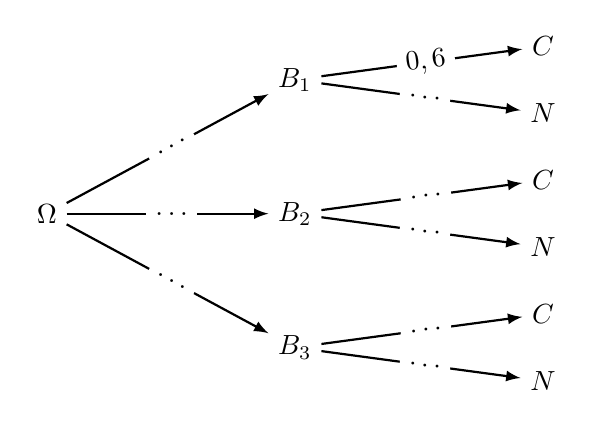
\begin{tikzpicture}
		\tikzstyle{fleche}=[->,>=latex,thick]
		\tikzstyle{noeud}=[]
		\tikzstyle{feuille}=[]
		\tikzstyle{etiquette}=[pos=0.52,sloped,fill=white]
		\def\DistanceInterNiveaux{3}
		\def\DistanceInterFeuilles{1}
		\def\NiveauA{(0)*\DistanceInterNiveaux}
		\def\NiveauB{(1.05)*\DistanceInterNiveaux}
		\def\NiveauC{(2.1)*\DistanceInterNiveaux}
		\def\InterFeuilles{(-0.85)*\DistanceInterFeuilles}
		\node[noeud] (R) at ({\NiveauA},{(2.5)*\InterFeuilles}) {$\Omega$};
		\node[noeud] (Ra) at ({\NiveauB},{(0.5)*\InterFeuilles}) {$B_1$};
		\node[feuille] (Raa) at ({\NiveauC},{(0)*\InterFeuilles}) {$C$};
		\node[feuille] (Rab) at ({\NiveauC},{(1)*\InterFeuilles}) {$N$};
		\node[noeud] (Rb) at ({\NiveauB},{(2.5)*\InterFeuilles}) {$B_2$};
		\node[feuille] (Rba) at ({\NiveauC},{(2)*\InterFeuilles}) {$C$};
		\node[feuille] (Rbb) at ({\NiveauC},{(3)*\InterFeuilles}) {$N$};
		\node[noeud] (Rc) at ({\NiveauB},{(4.5)*\InterFeuilles}) {$B_3$};
		\node[feuille] (Rca) at ({\NiveauC},{(4)*\InterFeuilles}) {$C$};
		\node[feuille] (Rcb) at ({\NiveauC},{(5)*\InterFeuilles}) {$N$};
		\draw[fleche] (R)--(Ra) node[etiquette] {$\ldots$};
		\draw[fleche] (Ra)--(Raa) node[etiquette] {$\num{0,6}$};
		\draw[fleche] (Ra)--(Rab) node[etiquette] {$\ldots$};
		\draw[fleche] (R)--(Rb) node[etiquette] {$\ldots$};
		\draw[fleche] (Rb)--(Rba) node[etiquette] {$\ldots$};
		\draw[fleche] (Rb)--(Rbb) node[etiquette] {$\ldots$};
		\draw[fleche] (R)--(Rc) node[etiquette] {$\ldots$};
		\draw[fleche] (Rc)--(Rca) node[etiquette] {$\ldots$};
		\draw[fleche] (Rc)--(Rcb) node[etiquette] {$\ldots$};
	\end{tikzpicture}
\end{center}

\begin{enumerate}
	\item Exprimer par une phrase l'information donnée par le nombre \num{0,6} sur la branche de $B_1$ à $C$.
	\item Compléter l'arbre pondéré ci-dessus.
	\item Définir par une phrase l'évènement $B_1 \cap C$ et calculer sa probabilité.
	\item Montrer que la probabilité $P(C)$ d'avoir un cookie au chocolat est égale à $\num{0,543}$.
	\item Calculer la probabilité d'avoir un cookie provenant de la boulangerie 2 sachant qu'il est au chocolat. On donnera le résultat arrondi au millième.
	\item Les évènements $B_2$ et $C$ sont-ils indépendants ? Justifier la réponse.
\end{enumerate}

\pagebreak

\exonum{4}

\medskip

On considère la fonction $f$ définie sur $\intervFF{-2}{4}$ par $f(x)=4x^3-9x^2-12x+6$.

On appelle $\mathscr{C}_f$ sa courbe représentative dans un repère orthogonal.

\begin{enumerate}
	\item Déterminer $f'(x)$.
	\item Étudier le signe de $f'(x)$ sur $\intervFF{-2}{4}$.
	\item Dresser le tableau de variations de la fonction $f$ sur $\intervFF{-2}{4}$.
	\item Tracer, dans le repère suivant, la courbe $\mathscr{C}_f$.
	\begin{center}
		\tunits{2.2}{0.11}
		\tdefgrille{-2}{4}{0.5}{0.25}{-40}{70}{10}{5}
		\begin{tikzpicture}[x=\xunit cm,y=\yunit cm]
			\tgrilles ; \tgrillep ;
			\axestikz* ; 
			\axextikz{-2,-1.5,-1,-0.5,0.5,1,1.5,2,2.5,3,3.5} ; 
			\axeytikz{-40,-30,-20,-10,10,20,30,40,50,60} ;
			\draw (0,0) node[below left=2pt] {$0$} ;
			\clip (\xmin,\ymin) rectangle (\xmax,\ymax) ;
			%\draw[very thick,red,samples=250,domain=\xmin:\xmax] plot (\x,{4*\x*\x*\x-9*\x*\x-12*\x+6}) ;
		\end{tikzpicture}
	\end{center}
\end{enumerate}

\medskip

\exogenerique{Question \faPython}{Bonus}

\medskip

On donne l'algorithme suivant, en langage \calgpython.

\begin{envpython}[12cm]
def mystere():
	u = 1500
	n = 0
	while u < 3000 :
		u = u * 1.04
		n = n + 1
	return n
\end{envpython}

\begin{enumerate}
	\item Expliquer brièvement ce que cet algorithme permet de faire.
	\item Que renverra la commande \cpy{mystere()} ? Justifier la réponse.
\end{enumerate}

\end{document}